%Version 3.1 December 2024
%% REVISED MANUSCRIPT for Automated Software Engineering (ASE) — revision of submission
%% "Scaling vs. Architecture: An Evaluation of SLMs for Automated Docstring Generation"
%% Paste into Overleaf as the single main .tex (all figures attached separately).

\documentclass[pdflatex,sn-mathphys-ay]{sn-jnl}% Math and Physical Sciences Numbered Reference Style

%%%% Standard Packages
\usepackage{graphicx}%
\graphicspath{{./bst/}}
\usepackage{multirow}%
\usepackage{amsmath,amssymb,amsfonts}%
\usepackage{amsthm}%
\usepackage{mathrsfs}%
\usepackage[title]{appendix}%
\usepackage{xcolor}%
\usepackage{textcomp}%
\usepackage{manyfoot}%
\usepackage{booktabs}%
\usepackage{algorithm}%
\usepackage{algorithmicx}%
\usepackage{algpseudocode}%
\usepackage{listings}%

\theoremstyle{thmstyleone}%
\newtheorem{theorem}{Theorem}%
\newtheorem{proposition}[theorem]{Proposition}%
\theoremstyle{thmstyletwo}%
\newtheorem{example}{Example}%
\newtheorem{remark}{Remark}%
\theoremstyle{thmstylethree}%
\newtheorem{definition}{Definition}%

\newcommand{\rev}[1]{{\color{blue}#1}}  %% revision highlighting; remove for camera-ready
\raggedbottom

\begin{document}

%% RETITLED (R2.9, R3.4): one-word change from the submitted title, adopting
%% Reviewer 2's own proposed wording ("capacity ... vs. architecture").
\title[Capacity vs. Architecture in SLM Docstring Generation]{Capacity vs.\ Architecture: An Evaluation of SLMs for Automated Docstring Generation}

\author*[1]{\fnm{Balaji} \sur{Venktesh}}\email{balaji23610040@snuchennai.edu.in}

\author*[1]{\fnm{Amsaprabhaa} \sur{M}}\email{amsaprabhaam@snuchennai.edu.in}

\author[1]{\fnm{Gireesh} \sur{Sundaram}}\email{gireesh23610036@snuchennai.edu.in}

\affil*[1]{\orgdiv{Department of Computer Science and Engineering}, \orgname{Shiv Nadar University}, \orgaddress{\city{Chennai}, \state{Tamilnadu}, \country{India}}}

%% ABSTRACT — fully rewritten. Changes vs. submitted version:
%% (a) model identities corrected: Llama 3.2 3B (not "8B"), Qwen3 (not "Qwen2.5"); range 3B–14B;
%% (b) honest scale: 67 curated classes, 2,613 core generations + ablation/validation runs;
%% (c) statistics from mixed-effects models at the per-class unit of analysis (R2.3);
%% (d) faithfulness judged against source code for all strategies (R2.2);
%% (e) blind two-annotator human validation replaces the withdrawn r=0.925 claim (R2.6);
%% (f) few-shot claim inverted by the dynamic-exemplar ablation (R2.8);
%% (g) LLM-judge reliability findings reported as a contribution (R1.4).
\abstract{\color{blue}
Automated docstring generation is a high-fidelity software engineering task in which factual correctness and efficiency are critical for local, resource-constrained deployment. We present a controlled, human-validated evaluation of 13 generation strategies across three open-weight Small Language Models (SLMs) spanning 3B--14B parameters (Llama~3.2~3B, Qwen3~8B, and Phi-4~14B), crossing four architectural families---Plain LLM, Few-Shot, Retrieval-Augmented Generation (RAG), and Iterative Critique RAG---with four reasoning-mode prompt variants (Base, CoT-, ToT-, and GoT-style structured decomposition). The core benchmark comprises 67 curated Python classes from TensorFlow/Keras and scikit-learn (2,613 core generations), extended by ablations of exemplar selection, retrieval-corpus relevance, quantization precision, and run-to-run variance, and evaluated with linear mixed-effects models at the per-class unit of analysis.

Our findings revise several common assumptions. First, model capacity is the dominant quality factor: Phi-4~14B and Qwen3~8B significantly outperform Llama~3.2~3B on both code-referenced faithfulness ($+0.047$ and $+0.064$, $p<0.001$) and semantic similarity, while no retrieval or critique architecture yields a significant faithfulness gain over zero-shot generation. Second, \emph{what} is retrieved matters more than \emph{whether} retrieval is used: retrieving structurally matched (code, docstring) exemplars outperforms the zero-shot baseline on every model ($+0.03$ to $+0.09$ BERTScore)---the strongest condition in the study---whereas retrieving documentation context yields only marginal gains even with a library-specific corpus. Third, GoT-style multi-axis decomposition is the only reasoning variant with a significant faithfulness benefit ($+0.032$, $p=0.003$), corroborated by blind human ratings, but costs $3.1\times$ latency; ToT-style branching costs $11.4\times$ with no benefit, and an FP16-vs-Q4 ablation shows quantization does not explain these results. Finally, we report a cautionary methodological finding: small LLM judges (DeepSeek-Coder~6.7B, Qwen3~8B) produce per-sample faithfulness scores that are unreliable across sampling draws and misaligned with strictly blind human judgment ($r\le 0.05$), despite agreeing almost perfectly with each other ($\rho=0.979$)---whereas reference-based metrics (rescaled BERTScore, pydocstyle adherence) validate well against humans. All claims in this paper rest on human-validated metrics and a blind two-annotator study (inter-rater ICC $=0.63$); we release the full benchmark, code, and evaluation artifacts.
}

\keywords{Small Language Models (SLMs), Automated Docstring Generation, Retrieval-Augmented Generation (RAG), LLM-as-a-Judge, Human Evaluation, Python}

\maketitle

\section{Introduction}
\label{intro}
Large Language Models (LLMs) have enabled substantial progress in software engineering tasks such as code generation, explanation, and summarization. To improve reliability, recent work increasingly augments LLMs with external context, explicit reasoning, and self-correction mechanisms. Among these approaches, Retrieval-Augmented Generation (RAG) has become a standard technique for grounding model outputs in external documentation rather than relying solely on parametric knowledge.

Automated docstring generation is a particularly important application of LLMs. Unlike open-ended summarization, docstring generation is a high-fidelity task in which generated descriptions must accurately reflect code behavior, parameters, and return values. Hallucinated or incorrect docstrings mislead human developers and propagate errors into downstream tooling that consumes code specifications, making this task a stringent benchmark for evaluating factual grounding in LLM-based systems~\cite{CanDR,gireesh}. While modern LLMs can produce fluent docstrings natively, standalone generation frequently yields generic or hallucinatory descriptions, especially for unfamiliar or domain-specific code~\cite{beyond}. Prior work therefore adopts RAG-based approaches that ground generation in style guides, API documentation, and coding conventions~\cite{codereview}. Figure~\ref{fig:rag-vs-no-rag} illustrates the qualitative difference between docstrings generated with and without external context.

Concurrently, recent research emphasizes generation-time reasoning strategies---such as Chain-of-Thought (CoT)~\cite{cot}, Tree-of-Thought (ToT)~\cite{tot}, Graph-of-Thought (GoT)~\cite{got}, and agentic self-correction---as general remedies for hallucination. These techniques show strong gains on tasks requiring multi-step planning and are increasingly applied to code documentation pipelines. This trend raises a critical but under-examined question for researchers and practitioners: \textbf{is the computational overhead of explicit reasoning or retrieval pipelines justified for documentation tasks that are structurally simple and context-bound, or is the parametric capacity of modern pretrained models alone sufficient for high-fidelity generation?}

The motivation for focusing on the Small Language Model (SLM) regime is the practicality of local, resource-constrained deployment: local execution is often a prerequisite in enterprise environments to preserve codebase privacy and avoid the latency and cost of frontier-model APIs. If SLMs lack the capacity to benefit from complex branching logic, practitioners may be paying a ``Reasoning Tax'' with no measurable return. Resolving this requires evaluating the \textbf{efficiency--quality frontier}: which strategies offer the best trade-off between documentation faithfulness and inference latency.

{\color{blue}
We study this question with a controlled factorial benchmark of \textbf{13 generation strategies} formed by crossing four architectural families---Plain LLM, Few-Shot LLM, Simple RAG, and Iterative Critique RAG---with four reasoning-mode prompt variants (Base, and CoT-, ToT-, and GoT-style structured prompting; Section~\ref{sec:methodology} details how our single-pass implementations relate to the canonical algorithms). We evaluate three instruction-tuned open-weight models spanning distinct capacity tiers and training lineages: Llama~3.2~3B~\cite{grattafiori2024llama3herdmodels}, Qwen3~8B~\cite{yang2025qwen3technicalreport}, and Phi-4~14B~\cite{abdin2024phi4technicalreport}, all served locally via Ollama with fixed generation parameters. The core benchmark comprises \textbf{67 curated Python classes} (Section~\ref{sec:dataset}) evaluated under all 39 model--strategy conditions (2,613 core generations), extended by targeted ablations---dynamic exemplar retrieval, retrieval-corpus relevance, FP16-vs-Q4 quantization, corrected critique gating, and repeated runs---that more than double the total number of generations.

A distinguishing feature of this study is its \emph{evaluation methodology}. All inferential claims derive from linear mixed-effects models with the benchmark class as a random effect, so identical classes evaluated under every condition are handled at the correct unit of analysis. Faithfulness is judged against the \emph{source code} as a single reference for all strategies, making scores commensurable across retrieval and non-retrieval families. Every automated metric is validated against a strictly blind human study: two annotators independently rated a stratified sample of 51 generated docstrings with all model scores hidden and item order shuffled (inter-rater ICC(2,1) $=0.63$). This validation shows that reference-based metrics (BERTScore with a strong rescaled backbone, and pydocstyle adherence) correlate substantially with blind human ratings ($r=0.52$ and $r=0.56$), whereas LLM-as-judge faithfulness scores do not (Section~\ref{sec:results}); our conclusions therefore rest on the human-validated metric suite.

Our analysis yields four cross-model findings:

\textbf{(1) Model capacity is the dominant quality factor.} Phi-4~14B and Qwen3~8B significantly outperform Llama~3.2~3B on code-referenced faithfulness ($+0.047$ and $+0.064$ respectively, both $p<0.001$) and on BERTScore ($+0.024$ and $+0.015$, both $p<0.001$), while no architectural family produces a significant faithfulness improvement over the zero-shot Plain LLM. Qwen3~8B matches or exceeds the twice-larger Phi-4 on several metrics, indicating that training quality partially compensates for scale; our design cannot fully separate the two, and we scope claims accordingly.

\textbf{(2) What you retrieve matters more than whether you retrieve.} Retrieving documentation context (the standard RAG recipe) yields marginal, mostly non-significant gains, even in an ablation with a library-specific corpus matched to the benchmark domains. In contrast, retrieving \emph{structurally matched (code, docstring) exemplars} for few-shot prompting outperforms the zero-shot baseline on every model ($+0.03$ to $+0.09$ BERTScore; ROUGE-1 nearly doubles)---the strongest condition in the study. A three-arm exemplar ablation shows that the poor performance of conventional static few-shot prompting is an artifact of structurally mismatched exemplars, not of in-context learning itself.

\textbf{(3) Structured multi-axis decomposition helps faithfulness; branching search does not.} The GoT-style variant is the only reasoning mode with a significant faithfulness benefit ($+0.032$, $p=0.003$), and blind human raters independently rank it highest among the strategies they evaluated---at a $3.1\times$ latency cost and a small significant BERTScore penalty ($-0.009$, $p=0.012$). The ToT-style variant costs $11.4\times$ latency with no significant benefit on any metric. An FP16-vs-Q4 quantization ablation shows these conclusions are not artifacts of 4-bit quantization.

\textbf{(4) Small LLM judges are not valid faithfulness evaluators for this task.} Per-sample scores from small LLM judges are dominated by sampling noise (identical inputs receive scores from 0.5 to 1.0 across draws), and even multi-draw-averaged scores from two judges of different families are misaligned with blind human judgment ($r\le0.05$) while agreeing almost perfectly with each other ($\rho=0.979$): both judges systematically over-rate retrieval- and critique-based outputs by $+0.2$--$0.3$ relative to blind human raters, rewarding retrieval-grounded fluency that humans do not. We recommend multi-draw averaging and strictly blind human validation as minimum methodological standards for LLM-as-judge evaluation, and detail the annotation-protocol sensitivity that motivates them in Section~\ref{sec:threats}.

Collectively, these findings indicate that for Python class-level docstring generation---a static, context-bound task---model selection and exemplar-based prompting dominate the efficiency--quality frontier, while documentation-retrieval pipelines and branching reasoning add cost without commensurate benefit at SLM scale. Beyond the empirical results, the paper contributes a fully released, cost-aware benchmark with human-validated evaluation, and a replicable demonstration of why LLM-as-judge scores require blind human validation before they can support scientific claims.


}
\section{Related Work}
\label{sec:related}

\subsection{Automated Code Documentation}
Automated code documentation, including summaries and docstrings, has been widely studied to improve software maintainability and developer productivity. Neural approaches to code summarization demonstrate that models trained jointly on code and natural language can generate fluent descriptions of program behavior. Recent efforts have demonstrated the utility of lightweight transformers, such as CodeT5, fine-tuned on synthetic datasets to automate function-level Python code summarization~\cite{Kharidu2025AutomatedFL}. While these specialized methods achieve strong performance on traditional token-overlap metrics, their capacity to generalize beyond their specific training distributions remains constrained. Similarly, Tao et al.~\cite{Tao2025RetrievalAugmentedCG} propose a retrieval-augmented summarization mechanism that integrates code semantics with dense representations, reflecting the evolution toward dynamic context retrieval. {\color{blue}
Reasoning-oriented prompting has also been applied directly to summarization: rethinking-based generation with a chain of comments progressively refines summaries through intermediate comment structures~\cite{chainofcomments2025}.

}
However, recent studies show that even strong code-specialized models frequently hallucinate undocumented parameters or behaviors when relying solely on parametric knowledge~\cite{CanDR,gireesh}. These findings motivate architectures that ground generation in external structural context---and raise the question of whether model pretraining quality alone may be sufficient for high-fidelity documentation tasks.

\subsection{Retrieval-Augmented Generation for Code Tasks}
Retrieval-Augmented Generation (RAG) improves factual grounding by injecting external, non-parametric information into LLM prompts at inference time. RAG has been studied in both general NLP summarization and code-related tasks. Zhang et al.~\cite{zhang-etal-2025-graph} introduce the Graph of Records, which enriches RAG by using historical LLM responses for long-context summarization, suggesting that richer context representations can benefit global documentation tasks. Several extensions to basic RAG---such as corrective retrieval, query reformulation, and source fusion---have been proposed~\cite{codereview}. However, evaluations in the literature overwhelmingly focus on single architectural variants, single foundation models, or surface-level text similarity metrics, {\color{blue}
and rarely vary the \emph{composition} of the retrieval corpus. This leaves open how reliability, computational efficiency, and structural faithfulness interact across diverse foundation models and corpus types---gaps our cross-model factorial evaluation and corpus ablation directly address.
}


\subsection{Advanced Reasoning Strategies for LLMs}
Beyond retrieval, explicit generation-time reasoning strategies have been introduced to improve LLM performance on complex tasks. Chain-of-Thought (CoT)~\cite{cot} prompts step-by-step rationale, while Tree-of-Thought (ToT)~\cite{tot} and Graph-of-Thought (GoT)~\cite{got} generate and aggregate multiple parallel reasoning paths through search and graph-structured aggregation. These methods show strong gains on planning and multi-step inference tasks, but their effectiveness for context-bound documentation tasks remains underexplored. {\color{blue}
We evaluate \emph{single-pass prompt-level adaptations} of these paradigms (Section~\ref{sec:reasoning-modes}); our ToT-style variant is related to Self-Consistency~\cite{wang2023selfconsistency} but synthesizes across structured decompositions targeting distinct documentation aspects rather than voting over equivalent outputs. All conclusions about these strategies in this paper are scoped to such prompt-level variants, not to the full search-based algorithms of the original works.
}


\subsection{Few-Shot and In-Context Learning for Code Tasks}
Few-shot prompting~\cite{brown2020languagemodelsfewshotlearners} enables models to adapt their outputs by conditioning on a small number of demonstrative examples, and has been applied to code generation~\cite{beyond} and retrieval-augmented settings~\cite{Izacard2022}. The intuition is that in-context examples of correctly formatted docstrings should guide the model toward PEP-compliant output structure, reducing reliance on architectural complexity. This intuition had not been systematically tested for class-level docstring generation, where the documentation target spans multiple methods, attributes, and inheritance structures. {\color{blue}
Our study evaluates three exemplar-selection regimes---static generic exemplars, persona-corrected static exemplars, and dynamically retrieved, structurally matched exemplars---directly testing whether exemplar relevance, rather than in-context learning per se, determines few-shot effectiveness.
}


\subsection{Evaluation of Code Summarization and LLM Outputs}
Standard n-gram metrics such as BLEU and ROUGE have historically been used to evaluate generated summaries, but correlate imperfectly with human judgments of documentation quality for generative LLMs that paraphrase rather than reproduce references~\cite{Sun2023AutomaticCS}. The LLM-as-a-Judge paradigm has emerged as a scalable alternative to human annotation~\cite{li-etal-2025-generation,bavaresco-etal-2025-llms}, yet its reliability varies substantially across task types and model families~\cite{bavaresco-etal-2025-llms}, {\color{blue}
and recent work shows that language models are poorly calibrated when assessing code summaries~\cite{calibrationcodesumm2025}.
Our study contributes direct evidence on this question: we quantify the per-sample draw variance of small LLM judges, test two judge families against a strictly blind two-annotator human study, and find that reference-based metrics---not LLM judges---align with human faithfulness judgment for this task (Section~\ref{sec:results}). This complements reported concerns about judge reliability with a task-specific validation protocol that other benchmark builders can reuse.
}


{\color{blue}
\subsection{Research Gap}
While prior work has independently advanced retrieval-augmented generation, reasoning-oriented prompting, few-shot prompting, and LLM-as-a-Judge evaluation, integrated empirical comparisons across multiple model families for high-fidelity documentation remain limited. Four gaps motivate our study:
\begin{enumerate}
  \item No prior work evaluates retrieval and reasoning strategies \emph{across} diverse modern open-weight models at the class level, leaving open whether architectural findings generalize beyond a single model.
  \item Exemplar selection for few-shot docstring generation has not been systematically compared against zero-shot and retrieval-based baselines.
  \item No prior study examines whether model capacity and training quality---independent of architectural choice---are the primary drivers of documentation quality.
  \item Benchmark studies in this space rarely validate their automated metrics against blind human judgment, leaving conclusions exposed to judge bias.
\end{enumerate}
Our study addresses all four through a controlled factorial benchmark across three SLMs (3B--14B), five targeted ablations, mixed-effects inference at the per-class level, and a blind two-annotator metric validation.


}
\section{Methodology}
\label{sec:methodology}

\subsection{Experimental Design}
We adopt a factorial experimental design that crosses four architectural families with four generation-time reasoning-mode prompt variants, yielding thirteen docstring generation strategies (Few-Shot uses Base mode only). This design enables controlled analysis of (i) retrieval versus no retrieval, (ii) the marginal utility of structured reasoning prompts, (iii) the effect of in-context demonstration, and (iv) the cost--benefit trade-offs of iterative self-correction, while holding all other variables constant. All strategies are implemented within a unified, configuration-driven framework. Figure~\ref{fig:architecture} shows the full experimental framework. Beyond the core grid, five ablations vary exemplar selection, retrieval-corpus composition, quantization precision, critique gating, and run-to-run seed (Section~\ref{sec:ablations-design}).
\begin{figure}[t]
    \centering
\includegraphics[width=1.0\linewidth,keepaspectratio]{architecture4.png}
    \caption{Experimental framework for Python docstring generation across three model families (Llama 3.2 3B, Qwen3 8B, Phi-4 14B). Four architectural families---Plain LLM, Few-Shot LLM, Simple RAG, and Iterative Critique RAG---combined with four reasoning-mode prompt variants (Base, CoT, ToT, GoT) yield thirteen strategies, all evaluated using shared quality, coverage, faithfulness, and computational cost metrics.}
    \label{fig:architecture}
\end{figure}

\subsection{Task Definition}
The target task is Python class-level docstring generation. Compared to function-level summarization, class docstrings require synthesizing information across methods, attributes, and inheritance structures, making the task particularly sensitive to hallucination and omission. Each model receives the raw source code of a class---with its original docstring removed---and generates a PEP-style docstring describing its purpose, parameters, attributes, return behavior, and potential exceptions. This setting reflects realistic documentation workflows and provides a stringent benchmark for evaluating factual grounding and interface completeness.

\subsection{Architectural Families}
We evaluate four architectural paradigms that represent increasing system complexity and prompting sophistication.
\paragraph{Plain LLM} serves as a no-retrieval baseline, relying solely on the model's parametric knowledge and the input source code.
\paragraph{Few-Shot LLM} extends the Plain LLM baseline by prepending two curated example (code, docstring) pairs to the prompt. {\color{blue}
In the interest of full transparency: post-submission code review found that the static few-shot prompt used in the core grid contained a copy-paste defect---its user message opened with an evaluator persona (``You are a strict technical judge\ldots'') conflicting with the writer persona in the system message. Rather than silently repairing the condition, we retain it as-run and add two ablation arms that isolate the defect from the exemplar-selection question: (a) a \emph{persona-corrected} static arm with identical exemplars, and (b) a \emph{dynamic} arm that retrieves the two most structurally similar other classes from the benchmark corpus (leave-one-out, by embedding similarity over the code) and uses their human-written docstrings as exemplars (Section~\ref{sec:ablations-design}; exemplar details in Appendix~\ref{sec:appendix-fewshot}).
}

\paragraph{Simple RAG} follows the standard retrieval-augmented generation paradigm~\cite{Lewis2020}. A dense retriever selects the top-$k$ relevant context chunks from an indexed corpus and concatenates them with the source code prior to generation.
\paragraph{Iterative Critique RAG} applies a test-time generate--critique--refine loop. The model first generates an initial docstring from the source code alone. A critique prompt then instructs the helper model (DeepSeek-Coder 6.7B) to assess the draft on four dimensions---\textit{Completeness}, \textit{Accuracy}, \textit{Formatting}, and \textit{Clarity} (0--2 points each)---and emit one of three labels: \textsc{excellent}, \textsc{good}, or \textsc{needs improvement} (Fig.~\ref{fig:iter-critique-prompt}). {\color{blue}
The rubric is prompt-embedded reasoning guidance; the runtime applies a substring check on the critique response rather than parsing a numeric score. \emph{As run in the core grid}, the check was \texttt{if "GOOD" not in response.upper()}: responses containing the substring \texttt{GOOD} bypassed retrieval, and all others triggered a single retrieval-augmented refinement pass. (The originally submitted manuscript misdescribed this gate as keyed on \texttt{EXCELLENT}; we correct the description here.) Because free-form critique responses can defeat any substring heuristic---e.g., by echoing the label list or using negated phrasing---we additionally implemented a robust verdict parser (assessment-line extraction with label-list and negation handling) and re-ran the family under the corrected gate as an ablation; trigger rates and downstream quality are statistically indistinguishable from the as-run condition for the two larger models (Section~\ref{sec:results}), indicating the heuristic gate did not materially affect the reported results.
}
 The mean API call count of 2.8--3.1 per sample reflects that refinement is triggered on roughly half the samples. This heuristic self-correction approach is distinct from trained reflection-token frameworks such as SELF-RAG~\citep{Asai2023SelfRAGLT}.

\subsection{Reasoning-Mode Prompt Variants}
\label{sec:reasoning-modes}
Across the Plain, Simple RAG, and Iterative Critique families, we apply four prompting strategies that vary the structure of generation-time reasoning. {\color{blue}
We emphasize the scope of these implementations: they are \emph{single-pass, prompt-level adaptations} inspired by the cited paradigms, not the full multi-node search (ToT) or iterative graph-aggregation (GoT) algorithms of the original works. We retain the CoT/ToT/GoT labels to indicate lineage, and scope all conclusions to these variants. All prompts are reproduced in Appendix~\ref{sec:appendix-prompts}.
}

\paragraph{Base} uses direct zero-shot prompting without explicit reasoning instructions.
\paragraph{CoT-style} prompting~\cite{cot} elicits step-by-step analysis of code parameters and behaviors within delimited reasoning tags before the final docstring.
\paragraph{ToT-style} prompting~\cite{tot} decomposes the documentation task into three sub-tasks, samples three candidates per sub-task, scores each candidate with the helper model, and synthesizes the best elements---a structured decompose-generate-select pipeline related to Self-Consistency~\cite{wang2023selfconsistency}, at roughly 14 model calls per sample.
\paragraph{GoT-style} prompting~\cite{got} analyzes the code independently along four axes---parameters, returns, functionality, and exceptions---and aggregates the analyses into a unified docstring, at roughly 4--5 model calls per sample.

{\color{blue}
\subsection{Evaluation Framework}
\label{sec:eval-design}
We employ a multi-dimensional evaluation framework in which every automated metric is validated against a blind human study (Section~\ref{sec:human-validation}), and metrics are weighted by that validation.
\paragraph{Human-validated primary metrics.} \textbf{BERTScore}~\cite{BERT} is computed with a \texttt{roberta-large} backbone and baseline rescaling (correlation with blind human faithfulness ratings: $r=0.52$); we additionally report the legacy \texttt{bert-base-uncased} scores for continuity ($r=0.47$) and note that strategy orderings are backbone-robust. \textbf{Pydocstyle adherence} measures PEP-257 conformance ($r=0.56$, the strongest human proxy in our validation). \textbf{ROUGE-1}~\cite{rouge} ($r=0.40$) and BLEU~\cite{BLEU} are reported as lexical-overlap references.
\paragraph{Descriptive metrics.} Parameter, Return, and Exception Coverage quantify whether interface elements are documented; conciseness measures information density against the reference. These correlate weakly with human faithfulness judgment ($|r|<0.17$) and are reported descriptively, not used for inferential claims.
\paragraph{LLM-as-a-Judge faithfulness (supplementary).} A judge model evaluates whether each statement in the generated docstring is supported by the \emph{source code}---the single reference for all thirteen strategies, making scores commensurable across retrieval and non-retrieval families. Because single judge draws at sampling temperature are unreliable (Section~\ref{sec:results}), each sample is scored as the mean of $k{=}3$ independent draws, and we report two judges from different families (DeepSeek-Coder 6.7B and Qwen3 8B). Judge scores failed blind human validation in our study and are therefore treated as supplementary throughout; we report them both for continuity with prior work and as the basis of our judge-reliability findings. A secondary token-overlap score against retrieved context is reported in Appendix~\ref{sec:appendix-token-overlap}.

\subsection{Blind Human Validation Protocol}
\label{sec:human-validation}
We validate all automated metrics against human judgment on a stratified sample of $N{=}51$ generated docstrings spanning all three SLMs and five representative strategies (Plain LLM Base, Simple RAG, Iterative Critique RAG, Plain LLM + CoT, Plain LLM + GoT). Two annotators independently rated every item. To eliminate anchoring, the annotation sheets contain \emph{only} the class source code and the generated docstring---no model identities, no strategy labels, and no automated metric values---and item order is independently shuffled per annotator; the key mapping items back to conditions is kept in a separate file opened only after both annotators finished. Each annotator assigned a continuous faithfulness score in $[0,1]$ judged against the source code. Inter-rater agreement is moderate-to-good (Pearson $r=0.62$, ICC(2,1) $=0.63$, MAE $=0.15$), and the mean of the two ratings serves as the human reference against which all automated metrics are validated (Section~\ref{sec:results}); full per-strategy results appear in Appendix~\ref{app:human-validation}. We additionally piloted a binary hallucination flag, whose chance-level inter-rater agreement ($\kappa=0.06$) led us to exclude it from analysis.

\subsection{Statistical Analysis}
\label{sec:stats-design}
Because all 67 benchmark classes are evaluated under every model--strategy condition, per-condition scores are not independent across conditions. All inferential claims therefore derive from linear mixed-effects models fitted on the per-class observations ($N{=}2{,}613$ per metric), with the benchmark class as a random intercept and architecture family, reasoning mode, and model as fixed effects (reference levels: Plain family, Base mode, Llama~3.2~3B), estimated by REML. The class random intercept is substantial (ICC $=0.28$ for BERTScore), confirming that class identity induces the dependence this design accounts for. We report fixed-effect estimates with Wald $p$-values and 95\% confidence intervals; coverage metrics are reported descriptively.

\subsection{Ablation Designs}
\label{sec:ablations-design}
Five ablations complement the core grid. \textbf{(a) Exemplar selection:} the three-arm few-shot comparison described above, run on all three models. \textbf{(b) Retrieval-corpus relevance:} Simple RAG re-run with a \emph{library-specific} corpus built from the benchmark libraries' developer guides and API-convention documentation (Keras subclassing and base-layer guides, scikit-learn developer documentation; per-class API reference pages are excluded to prevent leakage of ground-truth docstrings), holding the entire pipeline identical except the indexed corpus. \textbf{(c) Quantization:} the NoRAG family re-run at FP16 on Qwen3~8B and compared against the Q4\_K\_M default, testing whether 4-bit quantization suppresses reasoning benefits. \textbf{(d) Critique gating:} the Iterative Critique family re-run with the robust verdict parser. \textbf{(e) Run-to-run variance:} representative strategies repeated three times at the study's sampling temperature to quantify stability of quality and cost estimates.


}
\subsection{Reproducibility}
All experiments are driven by centralized configuration files that fix retrieval parameters, prompt templates, model settings, and evaluation criteria across all strategies. Hyperparameters are held constant across runs: retrieval uses $k=3$ top chunks, documents are segmented into 1,000-token chunks with 200-token overlap, and the embedding model is all-MiniLM-L6-v2 (384 dimensions). {\color{blue}
All prompts, configuration files, evaluation scripts, per-sample outputs, judge scores, and the blind-annotation artifacts are released in the project repository\footnote{\label{git}\url{https://github.com/balajivenky06/RAG-Docstring}}.
}


\section{Experimental Setup}
\label{sec:setup}

\subsection{Dataset}
\label{sec:dataset}
{\color{blue}
The benchmark comprises \textbf{67 curated Python classes} drawn from established open-source libraries: 45 from TensorFlow/Keras~\citep{tensorflow2015-whitepaper} (layers, optimizers, metrics, callbacks), 21 from scikit-learn~\citep{scikit-learn} (estimators, transformers, mixture models), and one general utility class (Table~\ref{tab:dataset-stats}). The corpus deliberately trades breadth for structural depth and evaluation intensity: classes range from shallow containers to deep inheritance hierarchies (66 of 67 classes use inheritance; mean 5.6 methods per class, maximum 34; median 119 lines, maximum 1{,}096), and every generated docstring in the study is scored under a nine-metric framework whose components are themselves validated against a blind two-annotator human study covering the majority of experimental cells. We view the resulting benchmark as complementary to larger, shallower corpora; scale-up to a substantially larger class corpus is left to future work, and all conclusions are scoped accordingly (Section~\ref{sec:threats}).


}
As illustrated in Fig.~\ref{fig:dataset}, the pipeline collects Python class files from public GitHub repositories and parses each into two aligned artifacts: (i) the raw class source code and (ii) its original developer-written docstring. To enforce a \emph{blind generation} setting, the docstring is removed from the input code before generation; the extracted docstring is retained verbatim as the reference annotation. Class names are anonymized to \texttt{dummy\_class\_1} in the cleaned variant consumed by the Plain LLM and Few-Shot strategies, preventing recall of memorized documentation for a named class.
\begin{figure}[t]
    \centering
    \includegraphics[width=1.0\linewidth]{dataset_creation_2.png}
    \caption{Dataset construction pipeline. Python classes are collected from GitHub, parsed to separate code and docstrings, and stripped of docstrings to create a blind generation setting; the extracted docstrings are used as reference annotations in the benchmarking framework (Fig.~\ref{fig:architecture}).}
    \label{fig:dataset}
\end{figure}

{\color{blue}
\begin{table}[h]
\centering
\small
\caption{Composition and structural complexity of the 67 benchmark classes.}
\label{tab:dataset-stats}
\begin{tabular}{lcc}
\toprule
\textbf{Library} & \textbf{Classes} & \textbf{\%} \\
\midrule
TensorFlow / Keras (layers, optimizers, metrics, callbacks) & 45 & 67.2\% \\
scikit-learn (estimators, transformers, mixtures) & 21 & 31.3\% \\
Other utilities & 1 & 1.5\% \\
\midrule
\textbf{Total} & \textbf{67} & \textbf{100\%} \\
\midrule
\multicolumn{3}{l}{\textit{Methods/class: mean 5.6, median 4, max 34; lines/class: median 119, max 1,096;}} \\
\multicolumn{3}{l}{\textit{classes using inheritance: 66/67.}} \\
\bottomrule
\end{tabular}
\end{table}


}
\subsection{Models and Infrastructure}
\label{sec:models-hardware}
{\color{blue}
To disentangle the contributions of architectural family and reasoning mode from parametric capacity, we evaluate three instruction-tuned open-weight models spanning distinct capacity tiers and training lineages, served via Ollama under the following exact tags:
\begin{itemize}
    \item \textbf{Llama~3.2~3B} (\texttt{llama3.2:latest})~\citep{grattafiori2024llama3herdmodels}: Meta's dense 3B-parameter transformer; the lightweight tier.
    \item \textbf{Qwen3~8B} (\texttt{qwen3:8b})~\citep{yang2025qwen3technicalreport}: Alibaba's 8B-parameter hybrid thinking/non-thinking model, evaluated in standard (non-thinking) mode; the mid tier.
    \item \textbf{Phi-4~14B} (\texttt{phi4:14b})~\citep{abdin2024phi4technicalreport}: Microsoft's 14B-parameter model trained on curated synthetic data with an emphasis on reasoning and code quality; the upper tier.
\end{itemize}
Generation parameters are fixed across every condition: temperature $=0.5$, top-$p=0.9$, \texttt{max\_tokens} $=2{,}048$, Q4\_K\_M quantization (an FP16 ablation tests sensitivity to precision; Section~\ref{sec:results-ablations}). A separate instance of \textbf{DeepSeek-Coder 6.7B} (\texttt{deepseek-coder:6.7b})~\citep{deepseekcoderv2} serves as the critique helper and as one of two LLM judges; \textbf{Qwen3 8B} additionally serves as a second, cross-family judge. The \texttt{all-MiniLM-L6-v2} encoder~\citep{reimers-gurevych-2019-sentence} (384 dimensions) provides dense embeddings for retrieval and exemplar matching, chosen to reflect realistic developer-tooling constraints.

All experiments ran on cloud GPU nodes (NVIDIA A100-SXM4-40GB, Ollama backend). We characterize this as \emph{local server-side inference}---the models are small enough for on-premises deployment on commodity server GPUs---rather than on-device execution; latency figures should be interpreted in that setting. Full hardware and serving details appear in Appendix~\ref{sec:appendix-hardware}.


}
\subsection{Retrieval Indexes}
\label{sec:retrieval-index}
The primary RAG knowledge base was constructed by scraping 21 authoritative generic Python documentation sources (PEP~257, the Google Python Style Guide, the pandas docstring guide, the NumPy/Napoleon Sphinx reference, and others; Appendix~\ref{sec:appendix-rag-corpus}), segmented into 1,000-token chunks with 200-token overlap, encoded with \texttt{all-MiniLM-L6-v2}, and stored in a Pinecone serverless index (cosine similarity). Each query retrieves the top-$k=3$ passages above a similarity threshold of $0.7$ under a 4,000-token context budget. {\color{blue}
The corpus-relevance ablation (Section~\ref{sec:ablations-design}) swaps in a \emph{library-specific} corpus of the benchmark libraries' developer guides and convention documentation under an identical retrieval interface.
}


\subsection{Execution Protocol}
\label{sec:protocol}
{\color{blue}
Table~\ref{tab:strategy-matrix} lists all 13 strategies in the $4$-family $\times$ $4$-mode factorial design (Few-Shot uses Base mode only). The core grid comprises
\[ 13\ \text{strategies} \times 3\ \text{models} \times 67\ \text{classes} = \mathbf{2{,}613}\ \text{core docstring generations,} \]
extended by the five ablations (exemplar selection, corpus relevance, FP16, corrected gating, repeated runs) to over $4{,}500$ generations in total, plus more than $15{,}000$ judge-scoring calls ($k{=}3$ draws $\times$ two judges over the core grid). No result caching or cross-condition reuse is permitted; every generation is produced independently. A subset of Llama ToT-family results was re-generated after an initial run showed inconsistent API-call counts; corrected values are used throughout. Alongside quality metrics, we record end-to-end wall-clock latency and model-call counts per sample. All prompts, hyperparameters, and evaluation settings are controlled via centralized configuration files\footref{git}.


}
\begin{table}[t]
\centering
\small
\setlength{\tabcolsep}{6pt}
\caption{The 13 experimental strategies spanning four architectural families and four reasoning-mode prompt variants. Few-Shot (S5) uses Base reasoning only.}
\begin{tabular}{clcc}
\toprule
\textbf{ID} & \textbf{Strategy Name} & \textbf{Family} & \textbf{Reasoning} \\
\midrule
S1  & Plain LLM                 & Plain           & Base \\
S2  & Plain LLM + CoT           & Plain           & CoT  \\
S3  & Plain LLM + ToT           & Plain           & ToT  \\
S4  & Plain LLM + GoT           & Plain           & GoT  \\
\midrule
S5  & Few-Shot LLM              & Few-Shot        & Base \\
\midrule
S6  & Simple RAG                & Simple RAG      & Base \\
S7  & Simple RAG + CoT          & Simple RAG      & CoT  \\
S8  & Simple RAG + ToT          & Simple RAG      & ToT  \\
S9  & Simple RAG + GoT          & Simple RAG      & GoT  \\
\midrule
S10 & Iter.\ Critique RAG       & Iter.\ Critique & Base \\
S11 & Iter.\ Critique RAG + CoT & Iter.\ Critique & CoT  \\
S12 & Iter.\ Critique RAG + ToT & Iter.\ Critique & ToT  \\
S13 & Iter.\ Critique RAG + GoT & Iter.\ Critique & GoT  \\
\bottomrule
\end{tabular}
\label{tab:strategy-matrix}
\end{table}

{\color{blue}
\section{Results}
\label{sec:results}

We organize results around five research questions: metric validity (RQ0), model capacity (RQ1), architectural families (RQ2), reasoning modes (RQ3), and exemplar selection (RQ4), followed by computational cost and stability analyses. All inferential statements derive from the mixed-effects models of Section~\ref{sec:stats-design}.

%=============================================================
\subsection{RQ0: Which Automated Metrics Track Human Judgment?}
\label{sec:rq0}
%=============================================================
Because every downstream claim depends on metric validity, we first report the blind human validation (protocol in Section~\ref{sec:human-validation}). Table~\ref{tab:human-corr} shows the correlation of each automated metric with the mean of the two blind annotators' faithfulness ratings over the $N{=}51$ validation sample.

\begin{table}[h]
\centering
\small
\caption{Validation of automated metrics against strictly blind human faithfulness ratings ($N{=}51$; two annotators, inter-rater $r=0.62$, ICC(2,1) $=0.63$). LLM-judge scores are means of $k{=}3$ draws, judged against source code.}
\label{tab:human-corr}
\begin{tabular}{lcc}
\toprule
\textbf{Metric vs.\ blind human mean} & \textbf{Pearson $r$} & \textbf{Spearman $\rho$} \\
\midrule
Pydocstyle adherence                        & \textbf{0.56} & \textbf{0.59} \\
BERTScore (roberta-large, rescaled)         & 0.52          & 0.45 \\
BERTScore (bert-base)                       & 0.47          & 0.41 \\
ROUGE-1                                     & 0.40          & 0.37 \\
Parameter coverage                          & 0.16          & 0.17 \\
Return coverage                             & 0.11          & 0.10 \\
Conciseness                                 & 0.02          & 0.15 \\
Exception coverage                          & $-$0.04       & 0.01 \\
\midrule
LLM-Judge, DeepSeek-Coder 6.7B ($k{=}3$)    & $-$0.21       & $-$0.23 \\
LLM-Judge, Qwen3 8B ($k{=}3$)               & 0.05          & 0.03 \\
\bottomrule
\end{tabular}
\end{table}

Three observations structure the rest of the paper. First, reference-based metrics---pydocstyle adherence and BERTScore---are the strongest human proxies; we therefore treat them as primary. Second, coverage metrics carry little information about human-perceived faithfulness and are reported descriptively only. Third, \emph{both} LLM judges fail validation: DeepSeek-Coder correlates negatively and Qwen3 near zero with blind human ratings, despite the two judges agreeing almost perfectly with each other on strategy-level rankings (Spearman $\rho = 0.979$ across all 39 model$\times$strategy cells). The judges share a systematic criterion that is not human-aligned: both over-rate retrieval- and critique-based outputs by $+0.2$--$0.3$ relative to blind humans (e.g., Simple RAG: judge 0.86 vs.\ human 0.57; Iterative Critique: 0.85 vs.\ 0.54), rewarding fluent retrieval-grounded paraphrase that human raters penalize for loss of code-specific detail. Two protocol findings underpin these results: single judge draws at sampling temperature are dominated by noise (identical inputs receive scores from 0.5 to 1.0 across draws; per-sample test--retest correlation $\approx 0$), and constrained score-first prompting further destroys judge validity (validation correlation drops from $+0.96$ to $-0.22$ on identical samples when the judge must emit its score before its reasoning). We therefore use $k{=}3$-draw means, report judge-based results as supplementary, and rest all primary claims on the human-validated metrics; the underlying protocol experiments are detailed in Appendix~\ref{app:judge-reliability}.

%=============================================================
\subsection{RQ1: Model Capacity}
\label{sec:rq1}
%=============================================================
Model capacity is the dominant quality factor in the study. Table~\ref{tab:mixedeffects} reports the mixed-effects estimates for the two headline metrics over all $N{=}2{,}613$ core observations.

\begin{table}[h]
\centering
\small
\caption{Linear mixed-effects estimates ($N{=}2{,}613$ per-class observations; class random intercept; REML). Reference levels: Plain family, Base mode, Llama~3.2~3B. Judge-based faithfulness is supplementary (Section~\ref{sec:rq0}). $^{*}p{<}0.05$, $^{**}p{<}0.01$, $^{***}p{<}0.001$.}
\label{tab:mixedeffects}
\begin{tabular}{lcc}
\toprule
\textbf{Fixed effect} & \textbf{BERTScore} & \textbf{Faithfulness (judge, $k{=}3$)} \\
\midrule
Intercept                    & 0.588$^{***}$          & 0.737$^{***}$ \\
Family: Few-Shot             & $-$0.080$^{***}$       & $-$0.017 \\
Family: Simple RAG           & $-$0.006\;($p{=}.052$) & $-$0.011 \\
Family: Iter.\ Critique RAG  & $-$0.034$^{***}$       & $+$0.006 \\
Mode: CoT                    & $-$0.005               & $+$0.001 \\
Mode: ToT                    & $+$0.001               & $+$0.008 \\
Mode: GoT                    & $-$0.009$^{*}$         & $+$0.032$^{**}$ \\
Model: Qwen3 8B              & $+$0.015$^{***}$       & $+$0.064$^{***}$ \\
Model: Phi-4 14B             & $+$0.024$^{***}$       & $+$0.047$^{***}$ \\
\midrule
Class ICC                    & 0.28                   & 0.07 \\
\bottomrule
\end{tabular}
\end{table}

Both larger models significantly outperform Llama~3.2~3B on both metrics (all $p<0.001$), and the model effects exceed every architectural effect in magnitude on faithfulness. Notably, Qwen3~8B matches or exceeds the twice-larger Phi-4~14B on judge-based faithfulness ($+0.064$ vs.\ $+0.047$) and trails it slightly on BERTScore, indicating that training lineage and data quality contribute alongside raw parameter count. Because the three models differ in vendor, data, and recipe, this design supports a \emph{capacity/training-quality} conclusion rather than a pure scaling law; we scope the claim accordingly.

%=============================================================
\subsection{RQ2: Architectural Families and Retrieval}
\label{sec:rq2}
%=============================================================
No architectural family significantly improves faithfulness over the zero-shot Plain LLM (all family effects non-significant; Table~\ref{tab:mixedeffects}), and two families significantly \emph{reduce} BERTScore: the static Few-Shot condition ($-0.080$, $p<0.001$; analyzed in depth in Section~\ref{sec:rq4}) and Iterative Critique RAG ($-0.034$, $p<0.001$). Simple RAG is quality-neutral ($-0.006$, $p=0.052$).

\paragraph{Corpus relevance (ablation).}
A natural objection is that our generic style-guide corpus under-serves retrieval. The corpus ablation (Table~\ref{tab:corpus-ablation}) tests this with a library-specific corpus matched to the benchmark domains. Corpus relevance matters directionally---the library corpus improves on the generic corpus for every model, and repairs the parameter-coverage damage that generic-corpus retrieval causes on the smallest model (Llama: 0.34 $\rightarrow$ 0.51)---but even the matched corpus never exceeds the Plain LLM baseline by more than $+0.012$ BERTScore. Retrieval of documentation context is thus corpus-sensitive but marginal at best on this task.

\begin{table}[h]
\centering
\small
\caption{Retrieval-corpus ablation: Simple RAG with the generic style-guide corpus (as in the core grid) vs.\ a library-specific corpus, against the Plain LLM baseline. BERTScore (bert-base) / parameter coverage.}
\label{tab:corpus-ablation}
\begin{tabular}{lccc}
\toprule
\textbf{Model} & \textbf{Plain LLM} & \textbf{RAG (generic)} & \textbf{RAG (library)} \\
\midrule
Llama 3.2 3B & 0.595 / 0.63 & 0.564 / 0.34 & 0.594 / 0.51 \\
Qwen3 8B     & 0.608 / 0.61 & 0.593 / 0.60 & 0.611 / 0.69 \\
Phi-4 14B    & 0.610 / 0.64 & 0.615 / 0.60 & 0.622 / 0.65 \\
\bottomrule
\end{tabular}
\end{table}

\paragraph{Iterative critique.}
The critique loop's BERTScore penalty is consistent with its mechanism: the refinement pass moves outputs toward fluent, abstractive prose (its token-overlap with retrieved context is the lowest of the retrieval families; Appendix~\ref{sec:appendix-token-overlap}) and away from code-specific phrasing. Blind human raters rank Iterative Critique lowest among the five validated strategies (0.54 vs.\ 0.63 for Plain), while both LLM judges rank it highly---the clearest instance of the judge--human divergence of Section~\ref{sec:rq0}. The gate-fix ablation (Section~\ref{sec:results-ablations}) confirms these results are not artifacts of the critique-gate heuristic.

%=============================================================
\subsection{RQ3: Reasoning-Mode Prompt Variants}
\label{sec:rq3}
%=============================================================
GoT-style multi-axis decomposition is the only reasoning variant with a significant faithfulness benefit ($+0.032$, $p=0.003$), at the cost of a small significant BERTScore reduction ($-0.009$, $p=0.012$) and a $3.1\times$ mean latency penalty (36.9\,s vs.\ 11.8\,s for Plain). The blind human study independently corroborates the direction of the GoT effect: human raters score Plain+GoT highest among the five validated strategies (0.71 vs.\ 0.63 for Plain Base), making GoT the one architectural intervention whose benefit survives both the commensurable judge metric and blind human assessment. CoT-style prompting is quality-neutral on both metrics. ToT-style branching yields no significant benefit on any metric while incurring the study's largest cost---134.0\,s mean latency ($11.4\times$ Plain) and ${\approx}14$ model calls per sample---placing it strictly outside the Pareto frontier (Fig.~\ref{fig:efficiency_frontier}).

\paragraph{Quantization is not the explanation (ablation).}
To test whether 4-bit quantization suppresses reasoning benefits (a potential confound for any negative reasoning result), we re-ran the NoRAG family at FP16 on Qwen3~8B. Differences are uniformly small (BERTScore deltas: Plain $-0.004$, CoT $+0.005$, GoT $+0.007$, ToT $+0.004$, Few-Shot $+0.010$), an order of magnitude below the effects of interest, while FP16 substantially increases latency. The reasoning-mode conclusions are therefore not artifacts of quantization.

%=============================================================
\subsection{RQ4: Exemplar Selection for Few-Shot Prompting}
\label{sec:rq4}
%=============================================================
The static Few-Shot condition is the study's weakest ($-0.080$ BERTScore, $p<0.001$), with a distinctive degenerate-output signature: on Qwen3, 24 of 67 outputs (36\%) collapse to fewer than 10 words (median 12), and on Phi-4, 8 of 67. The three-arm exemplar ablation (Table~\ref{tab:fewshot-ablation}) decomposes this failure.

\begin{table}[h]
\centering
\small
\caption{Exemplar-selection ablation (BERTScore, bert-base / ROUGE-1 / median output words). \emph{Static} is the core-grid condition (with the disclosed persona defect); \emph{Static-fixed} corrects the persona with identical exemplars; \emph{Dynamic} retrieves the two most structurally similar other benchmark classes (leave-one-out) as exemplars. \textbf{Bold} = best per model.}
\label{tab:fewshot-ablation}
\begin{tabular}{lcccc}
\toprule
\textbf{Model} & \textbf{Plain LLM} & \textbf{Static} & \textbf{Static-fixed} & \textbf{Dynamic} \\
\midrule
Llama 3.2 3B & 0.595 / 0.169 / 159 & 0.577 / 0.149 / 111 & 0.504 / 0.124 / 24 & \textbf{0.636 / 0.288 / 152} \\
Qwen3 8B     & 0.608 / 0.206 / 114 & 0.455 / 0.089 / 12  & 0.530 / 0.151 / 46  & \textbf{0.694 / 0.390 / 151} \\
Phi-4 14B    & 0.610 / 0.201 / 96  & 0.531 / 0.134 / 39  & 0.591 / 0.197 / 107 & \textbf{0.671 / 0.375 / 161} \\
\bottomrule
\end{tabular}
\end{table}

Three conclusions follow. First, \textbf{dynamically retrieved, structurally matched exemplars outperform the zero-shot baseline on every model} ($+0.041$ to $+0.087$ BERTScore; ROUGE-1 roughly doubles), producing the strongest condition in the entire study (Qwen3/Dynamic, 0.694) and eliminating degenerate truncation. Second, the persona correction alone interacts with capacity: it substantially rescues Phi-4 (0.531 $\rightarrow$ 0.591, with the study's best parameter coverage, 0.74) and partially rescues Qwen3, but further degrades the 3B model, which responds to the cleaner instruction by imitating the terse exemplars even more literally. Third, combining these results with RQ2 (Section~\ref{sec:rq2}): the effective use of retrieval on this task is retrieving \emph{exemplars}, not \emph{documentation}---in-context learning is not harmful per se; mismatched static exemplars are. Because dynamic exemplars are drawn leave-one-out from sibling classes in the same libraries, part of the reference-similarity gain may reflect shared documentation conventions; we flag this in Section~\ref{sec:threats}.

%=============================================================
\subsection{Computational Cost}
\label{sec:cost2}
%=============================================================
Plain LLM requires a single model call and 7.1--18.8\,s per class depending on the model. Simple RAG adds one context-rewrite call; its latency is competitive for Llama and Phi-4 but degrades sharply for Qwen3 (110.5\,s vs.\ 18.8\,s), an \emph{output-verbosity effect}: Qwen3 elaborates on retrieved text in unstructured RAG prompts, while structurally constrained prompts (GoT: 33.7\,s; CoT: 44.4\,s) prevent open-ended elaboration. Iterative Critique averages 2.8--3.1 calls per sample. GoT-style prompting costs $3.1\times$ Plain latency on average; ToT-style costs $11.4\times$ with ${\approx}14$ calls per sample and is dominated on every quality metric---the ``Reasoning Tax'' in its clearest form. Figure~\ref{fig:latency_quality} and Figure~\ref{fig:efficiency_frontier} visualize the latency--quality trade-off and the call--quality frontier over all 39 model$\times$strategy cells.

\begin{figure}[t]
    \centering
    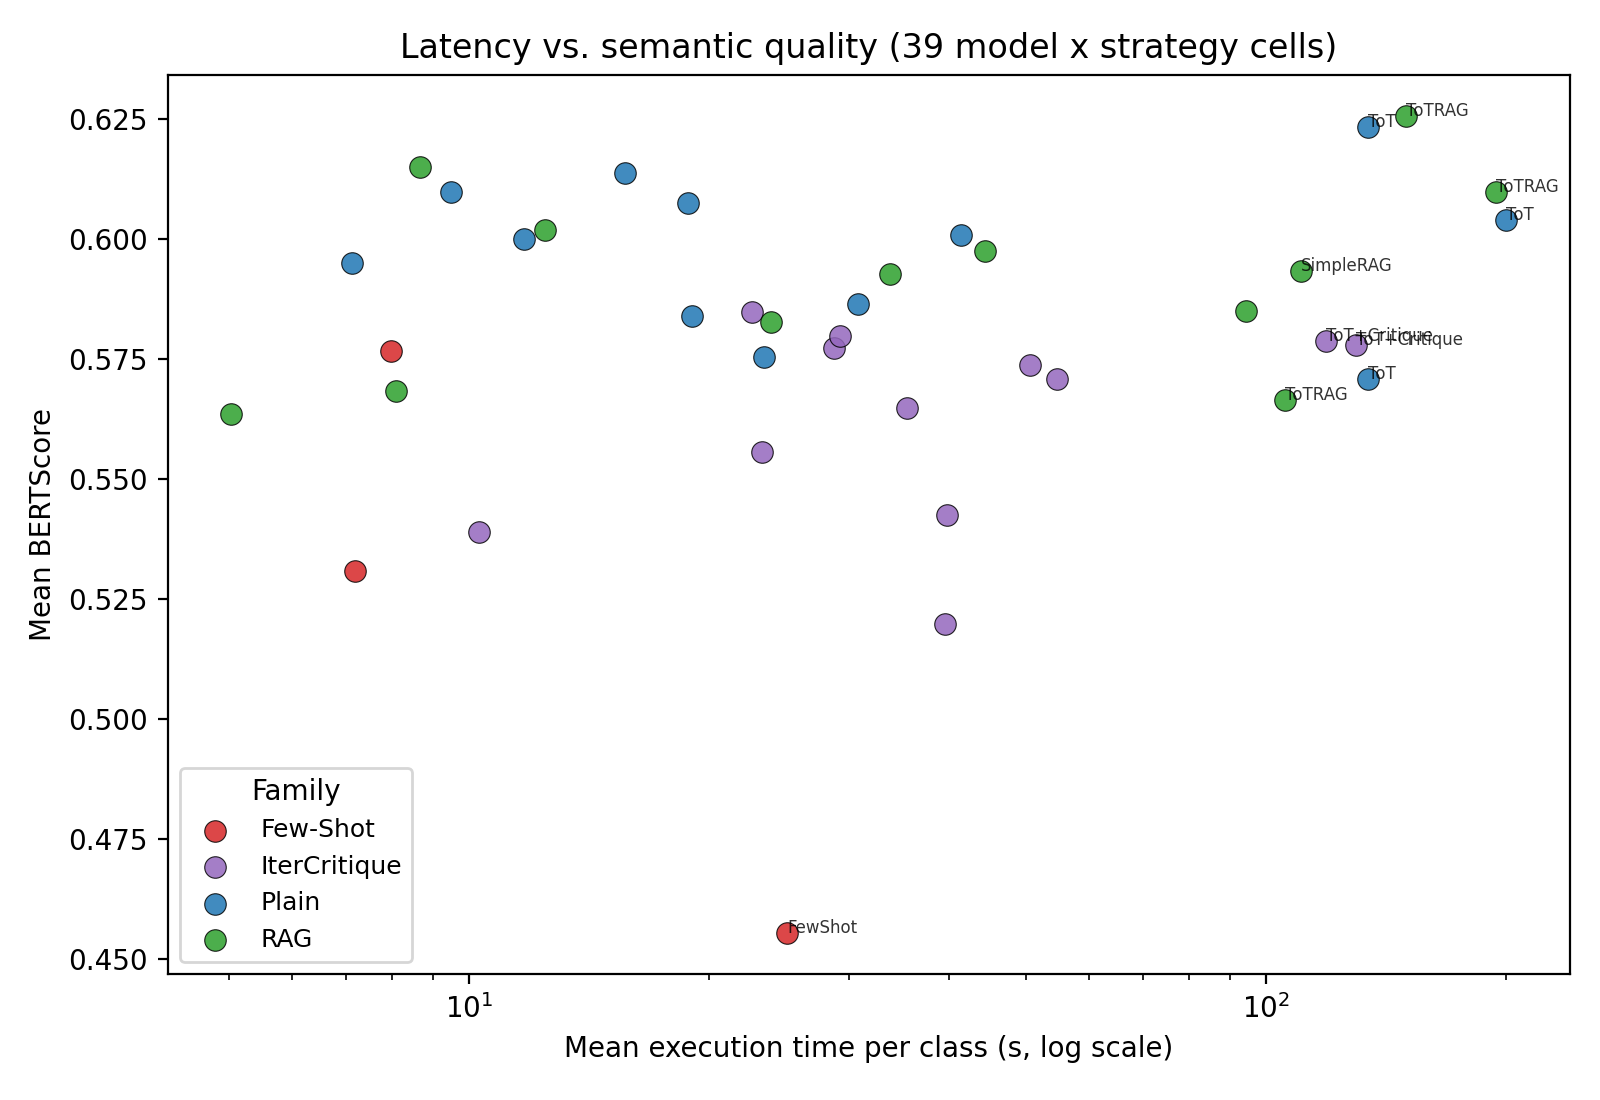
\includegraphics[width=\linewidth]{fig_latency_vs_bertscore.png}
    \caption{Latency--quality trade-off: mean execution time (s, log scale) versus mean BERTScore per model$\times$strategy cell, colored by architectural family. Upper-left is Pareto-optimal. ToT-style configurations cluster at the right (highest cost) with no quality advantage; the static Few-Shot conditions occupy the lower left.}
    \label{fig:latency_quality}
\end{figure}

\begin{figure}[t]
    \centering
    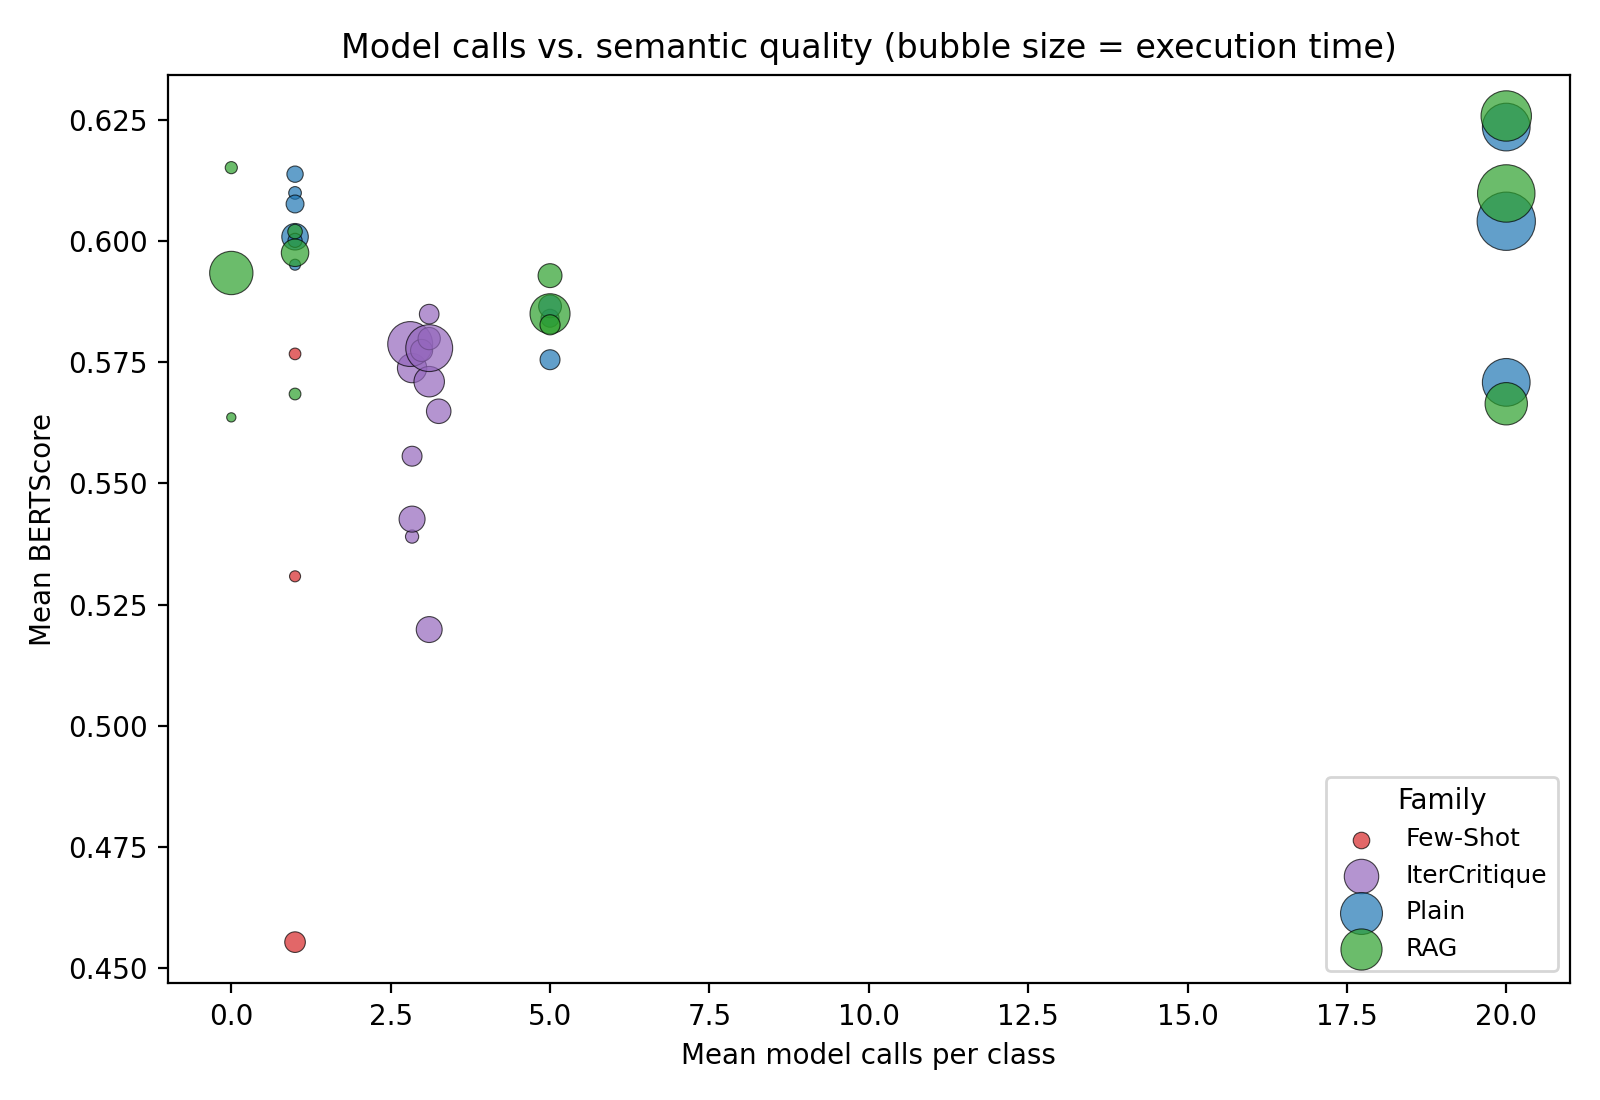
\includegraphics[width=\linewidth]{fig_calls_vs_bertscore.png}
    \caption{Efficiency frontier: mean model calls per class versus mean BERTScore; bubble size encodes mean execution time. Single-call zero-shot configurations sit on the frontier; ToT-style configurations ($\approx$14 calls) are dominated on both dimensions.}
    \label{fig:efficiency_frontier}
\end{figure}

%=============================================================
\subsection{Stability and Gate-Fix Ablations}
\label{sec:results-ablations}
%=============================================================
\paragraph{Run-to-run variance.} Repeating representative strategies three times at the study's sampling temperature yields highly stable strategy-level estimates: across-run standard deviations of mean BERTScore are $0.0015$ (Plain LLM) and $0.0017$ (Simple RAG)---one to two orders of magnitude below the effects of interest (Appendix~\ref{sec:appendix-variance}). Strategy-level means---the quantities all conclusions rest on---are robust to sampling stochasticity, in contrast to per-sample judge scores (Section~\ref{sec:rq0}).
\paragraph{Corrected critique gate.} Re-running the Iterative Critique family with the robust verdict parser leaves quality metrics within $\pm 0.01$ BERTScore and API-call counts within $\pm 0.2$ calls of the as-run condition on Phi-4 (all four modes) and Qwen3 (Base). On Llama~3.2~3B, the corrected gate modestly \emph{improves} the Base condition ($+0.036$ BERTScore, $+0.065$ parameter coverage, API calls unchanged at ${\approx}2.8$), consistent with the smallest model being most sensitive to which samples are selected for refinement; even so, the corrected condition remains below the Plain LLM baseline (0.575 vs.\ 0.595), so no reported conclusion depends on the gate heuristic.



}
{\color{blue}
\section{Discussion}
\label{sec:discussion}

\subsection{Why Reasoning Prompts Rarely Help: Mechanisms}
\label{sec:mechanisms}
Beyond the aggregate statistics, the per-sample outputs reveal three mechanisms that explain when and why architectural interventions fail on this task.

\paragraph{Hallucination by inference.}
Docstring generation is a descriptive, extractive task: the correct output faithfully restates information already present in the class definition. When a reasoning prompt instructs the model to ``think step by step about what this class could do,'' it activates generalized knowledge about the class \emph{type}, not just the specific code at hand. A concrete illustration: given a custom Keras layer whose \texttt{call()} method performs only a linear transformation, a ToT-style run generated \emph{``Applies dropout regularization during training to prevent overfitting''}---plausible for a generic Keras layer, and entirely unsupported by the presented source. Under Plain LLM generation the same class received a faithful description. Reasoning helps when its inferences align with the actual code and harms when it activates irrelevant parametric associations; across a heterogeneous benchmark the two effects largely cancel for CoT- and ToT-style prompting, while GoT's fixed four-axis decomposition---which constrains reasoning to \emph{enumerating what is present} (parameters, returns, functionality, exceptions) rather than speculating about behavior---retains a modest positive effect.

\paragraph{Format-compliance failures scale inversely with capacity.}
Structured prompting assumes the model can reliably execute the output format. The smallest model cannot, always: all five runaway generations in the study (repetition loops of $2{,}000$ to $290{,}000$ words) occurred in Llama~3.2~3B reasoning-mode conditions, where the model lost the delimiter format and the fallback captured an unterminated reasoning trace. No such failure occurred for the 8B and 14B models. Similarly, the static few-shot condition induced degenerate truncation (outputs under 10 words) in 36\% of Qwen3 samples and 12\% of Phi-4 samples. These failure modes are invisible in aggregate means yet account for much of the observed cross-condition variance, and they imply that prompt-level ``architecture'' presupposes a capacity floor---consistent with our headline finding that capacity dominates architecture.

\paragraph{Judges reward retrieval-grounded fluency; humans reward code specificity.}
The judge--human divergence of Section~\ref{sec:rq0} is systematic, not noise: both judges over-rate exactly the two families whose mechanism is to \emph{rewrite} content fluently (retrieval-conditioned generation and critique-driven refinement). Inspection of divergent samples shows the refinement pass smooths code-specific detail into well-formed generic prose; the judges score the fluent restatement as well-supported, while blind human raters penalize the loss of specificity. This bias inverts strategy rankings---the judges place Simple RAG and Iterative Critique near the top; blind humans place them at the bottom---and would have silently distorted our conclusions had the metrics not been validated.

\subsection{What You Retrieve Matters More Than Whether You Retrieve}
Our retrieval results seem contradictory at first: documentation-context RAG is quality-neutral at best (Section~\ref{sec:rq2}), yet exemplar retrieval is the study's strongest intervention (Section~\ref{sec:rq4}). The resolution is that the two retrieve different \emph{kinds} of information. Documentation context tells the model how docstrings should look in general---information that well-pretrained models already possess parametrically, which is why even a library-specific corpus adds little. Structurally matched exemplars instead show the model what a correct docstring looks like \emph{for a class shaped like this one}, supplying task-specific structure that generic pretraining cannot: the exemplar functions as an implicit output template fitted to the target's method count, inheritance profile, and parameter style. This reframes the practical question for retrieval-augmented documentation tooling from ``should we add RAG?'' to ``what should the index contain?''---and our evidence says: exemplar pairs, not style guides.

\subsection{Iterative Critique Does Not Substitute for External Verification}
The critique loop reduces BERTScore ($-0.034$, $p<0.001$), receives the lowest blind-human faithfulness rating among validated strategies, and lowers all coverage metrics descriptively---while costing $2.8$--$3.1$ model calls per sample. Since the critic and generator share the same context and inductive biases, self-correction tends to reinforce rather than resolve errors, and the refinement pass actively abstracts away the code-specific phrasing that humans value. For structured documentation tasks, verification needs an external signal (static analysis, signature checking) rather than model self-reflection.

\subsection{The Reasoning Tax, Revised}
The submitted version of this study framed all reasoning overhead as unjustified. The corrected, human-validated analysis supports a more nuanced position. GoT-style multi-axis decomposition delivers the study's only significant faithfulness gain, corroborated by blind human raters, at $3.1\times$ latency and a marginal semantic-similarity cost---a defensible trade wherever faithfulness dominates latency (e.g., documentation generated once and reviewed by humans). ToT-style branching remains a pure tax: $11.4\times$ latency, ${\approx}14$ model calls, no significant benefit on any metric, and the FP16 ablation rules out quantization as an excuse. The practitioner guidance is therefore not ``never reason'' but: choose the strongest model you can serve; add structured enumeration (GoT-style) when faithfulness is critical; use dynamically retrieved exemplars as the cheapest quality lever (one call, no added latency structure); and avoid branching search and self-critique loops at this scale.


}
{\color{blue}
\section{Threats to Validity}
\label{sec:threats}

\subsection{Internal Validity}
Two prompt-level defects in the core grid were found during post-submission code review and are disclosed in Section~\ref{sec:methodology}: the static few-shot prompt contained a conflicting persona, and the Iterative Critique gate was keyed on the substring \texttt{GOOD} rather than the documented \texttt{EXCELLENT}. Rather than silently repairing the record, we quantified both: the persona defect is dissected by the three-arm exemplar ablation (its correction alone does not rescue static few-shot, and interacts with model capacity), and the corrected-gate rerun leaves results statistically indistinguishable on the two larger models. A subset of Llama ToT-family results was re-generated after an initial run showed inconsistent API-call counts. All generation and retrieval parameters were otherwise held constant across conditions, and run-to-run repeats show strategy-level means are stable under sampling stochasticity.

The most consequential internal-validity finding of the revision concerns our own evaluation instruments. The human validation reported in the originally submitted manuscript ($r=0.925$ between annotator and judge) used annotation sheets that displayed the judge's scores alongside the entry field; a strictly blind re-annotation of the same 51 items by two annotators correlates only weakly with those original ratings ($r=0.16$) and with the judge ($r=0.13$), indicating the original ratings were anchored to the visible scores. We therefore withdrew the original validation and rebuilt all human-referenced claims on the blind study. We report this experience as a caution for the growing LLM-as-judge literature: agreement estimates obtained under non-blind protocols can be arbitrarily inflated, and per-sample judge scores at sampling temperature are draw-noise unless averaged.

\subsection{External Validity}
The benchmark is 67 Python classes concentrated in two ecosystems (TensorFlow/Keras 67\%, scikit-learn 31\%); generalization to other libraries, languages, documentation formats (JavaDoc, JSDoc), and finer-grained targets (method-level, module-level) is unverified. The depth-for-breadth trade-off is deliberate (Section~\ref{sec:dataset}) but limits population claims; replication on a larger, more diverse corpus is the most valuable extension of this work. We evaluate three open-weight models spanning 3B--14B served via Ollama; findings may not transfer to frontier-scale models or code-specialist fine-tunes. Because the three models differ in vendor and training recipe, capacity effects cannot be fully separated from training-quality effects; within-family scale comparisons would isolate the former.

\subsection{Construct Validity}
All primary claims rest on metrics validated against a blind human study, but that study is itself modest: $N=51$ items, five of thirteen strategies, two annotators with moderate agreement (ICC $=0.63$), and a hallucination flag too unreliable to use ($\kappa=0.06$). The dynamic-exemplar gains partially reflect shared documentation conventions between sibling classes of the same library; cross-library exemplar retrieval would separate structural matching from stylistic leakage. LLM-judge faithfulness is reported as supplementary only; developer-perceived usefulness in real IDE workflows was not assessed.

\subsection{Conclusion Validity}
Inferential claims derive from linear mixed-effects models at the per-class unit of analysis ($N=2{,}613$), which account for the dependence induced by evaluating identical classes under every condition (class ICC up to 0.28); Wald $p$-values are reported with the model structure fixed a priori. Coverage metrics are reported descriptively without significance claims. Effects smaller than ${\sim}0.01$ BERTScore may still escape detection at this sample size.

\section{Conclusion}
\label{sec:conclusion}
We presented a controlled, human-validated evaluation of 13 docstring-generation strategies across three open-weight SLMs spanning 3B--14B parameters, on a 67-class Python benchmark with 2,613 core generations, five targeted ablations, and mixed-effects inference at the per-class level.

Four findings emerge. First, \textbf{model capacity and training quality dominate architecture}: Qwen3~8B and Phi-4~14B significantly outperform Llama~3.2~3B on every validated metric, while no retrieval or critique architecture significantly improves faithfulness over zero-shot generation. Second, \textbf{the effective use of retrieval is exemplar retrieval}: structurally matched (code, docstring) exemplars outperform the zero-shot baseline on all three models---the study's strongest condition---whereas documentation-context RAG is marginal even with a domain-matched corpus, and the apparent harm of few-shot prompting in the core grid traces to static, mismatched exemplars rather than in-context learning itself. Third, \textbf{structured enumeration helps; branching search does not}: GoT-style decomposition yields the only significant faithfulness gain, corroborated by blind human raters, at $3.1\times$ latency, while ToT-style branching costs $11.4\times$ with no benefit, and quantization does not explain either result. Fourth, \textbf{small LLM judges are not valid faithfulness evaluators for this task}: two judge families agree with each other ($\rho=0.979$) while misaligning with blind human judgment ($r\le0.05$), systematically over-rating retrieval-grounded fluency---whereas reference-based metrics validate well.

For practitioners building local documentation tooling, the guidance is concrete: invest first in the strongest servable model; add dynamically retrieved exemplars (one extra retrieval, no latency structure); reserve GoT-style enumeration for faithfulness-critical settings; and avoid branching reasoning, critique loops, and unvalidated LLM-judge metrics. For researchers, the study demonstrates that benchmark conclusions can invert under metric validation---the case for strictly blind, multi-annotator validation of every automated evaluator, and for releasing the artifacts that let others check. Future work should replicate at larger corpus scale, extend to other languages and documentation granularities, isolate scale from training quality via within-family comparisons, and investigate whether larger judges pass blind validation.


}
\section*{Declarations}

\paragraph{Funding}
The authors did not receive support from any organization for the submitted work.

\paragraph{Competing Interests}
The authors have no competing interests to declare that are relevant to the content of this article.

\paragraph{Ethics Approval}
{\color{blue}
Not applicable. The human evaluation was performed by the authors as expert annotators and involved no external participants.
}


\paragraph{Consent to Participate}
Not applicable.

\paragraph{Consent for Publication}
The authors give their consent for the publication of details within this manuscript.

\paragraph{Data Availability}
{\color{blue}
The benchmark dataset, all per-sample generations, judge scores, blind-annotation sheets and key, and analysis outputs are available in the GitHub repository: \url{https://github.com/balajivenky06/RAG-Docstring}.
}


\paragraph{Code Availability}
The custom code used for generation, evaluation, ablations, and statistical analysis is available at: \url{https://github.com/balajivenky06/RAG-Docstring}.

\paragraph{Author Contributions}
All authors contributed to the study conception and design. Material preparation and data collection were performed by Balaji Venktesh. Evaluation and analysis were performed by Balaji Venktesh, Amsaprabhaa M, and Gireesh Sundaram. {\color{blue}
The two blind annotations were performed independently by two of the authors.
}
 The first draft of the manuscript was written by Balaji Venktesh, and all authors commented on previous versions of the manuscript. All authors read and approved the final manuscript.

\paragraph{Use of AI Tools}
%% [[NOTE TO AUTHORS: updated for accuracy — the original statement (copy-editing only)
%%    no longer reflects the revision process; please confirm wording.]]
{\color{blue}
The authors used an AI coding assistant during revision for code review, analysis scripting, and manuscript drafting support, under the direction of the authors. All experimental design decisions, data collection, human annotation, and conclusions were made and verified by the human authors, who take full accountability for the content and factual accuracy of the manuscript. All experiments used publicly available, open-source code and datasets under their respective licenses. No private, sensitive, or personally identifiable data were used.
}


\bibliography{sn-bibliography}

\appendix

%------------------------------------------------------------------
{\color{blue}
\section{Blind Human Validation Details}
\label{app:human-validation}
%------------------------------------------------------------------
Two annotators independently rated the same stratified sample of $N{=}51$ generated docstrings (three models $\times$ five strategies). Annotation sheets contained only the class source code and the generated docstring; item order was independently shuffled per annotator with different seeds, and the key mapping items to conditions was stored separately and opened only after both annotators finished. The sheets, key, and merged scores are released with the repository.

\begin{table}[h]
\centering
\small
\caption{Blind human study: agreement and per-strategy means. Judge columns are $k{=}3$-draw means judged against source code.}
\label{tab:blind-details}
\begin{tabular}{lcccc}
\toprule
\textbf{Strategy} & \textbf{$n$} & \textbf{Human mean} & \textbf{DeepSeek judge} & \textbf{Qwen3 judge} \\
\midrule
Plain LLM + GoT        & 9  & \textbf{0.71} & 0.91 & 0.41 \\
Plain LLM (Base)       & 12 & 0.63 & 0.68 & 0.28 \\
Plain LLM + CoT        & 9  & 0.62 & 0.78 & 0.41 \\
Simple RAG (Base)      & 12 & 0.57 & 0.86 & 0.39 \\
Iterative Critique RAG & 9  & 0.54 & 0.85 & 0.44 \\
\midrule
\multicolumn{5}{l}{Inter-rater: Pearson $r=0.62$; ICC(2,1) $=0.63$; MAE $=0.15$.} \\
\multicolumn{5}{l}{Hallucination flag: raw agreement 72.5\%, Cohen's $\kappa=0.06$ (excluded from analysis).} \\
\bottomrule
\end{tabular}
\end{table}

Both judges apply strategy orderings nearly opposite to the human ordering (judges: retrieval/critique families high; humans: low), and the two judges' absolute scales differ by $0.3$--$0.4$ while their strategy-level rankings agree ($\rho=0.979$ over all 39 cells)---absolute LLM-judge scores are judge-dependent and should not be compared across studies.

%------------------------------------------------------------------
\section{LLM-Judge Reliability Protocols}
\label{app:judge-reliability}
%------------------------------------------------------------------
Three protocol experiments underlie the judge findings of Section~\ref{sec:rq0}.
\textbf{(a) Draw variance:} scoring the identical (code, docstring) pair five times at sampling temperature yields scores spanning 0.5--1.0 (example draws: 0.9, 1.0, 0.75, 0.5, 0.6); across the full grid, the per-sample correlation between two independent scoring passes of unchanged conditions is ${\approx}0$, while strategy-level means over 67 classes shift by only $0.03$--$0.09$.
\textbf{(b) Output-format sensitivity:} constraining the judge to emit its score on the first line with a capped token budget (a common efficiency practice) collapsed validation correlation on identical samples from $r=+0.96$ to $r=-0.22$; reasoning-before-scoring is load-bearing for judge quality.
\textbf{(c) Reference commensurability:} in the originally submitted pipeline, RAG-family outputs were judged against retrieved context while No-RAG outputs were judged against source code, making cross-family comparisons non-commensurable; all judge scores in this paper use source code as the single reference for every strategy.

%------------------------------------------------------------------

}
\section{Token-Overlap Faithfulness Scores}
\label{sec:appendix-token-overlap}
%------------------------------------------------------------------
A secondary token-overlap score is computed for retrieval-based strategies as
$\text{Token-Overlap} = |D_{\text{tokens}} \cap RC_{\text{tokens}}| / |D_{\text{tokens}}|$,
where $D_{\text{tokens}}$ are content tokens of the generated docstring and $RC_{\text{tokens}}$ tokens of the retrieved context (stopwords removed). Simple RAG achieves the highest overlap (mean 0.331), confirming that direct retrieval-grounded generation stays closest to retrieved phrasing; Iterative Critique strategies score lowest within the retrieval group (0.217--0.254), indicating the critique loop shifts generation toward abstractive restatements. {\color{blue}
This abstraction is precisely the behavior that LLM judges reward and blind human raters penalize (Section~\ref{sec:mechanisms}); token-overlap thus serves as a useful \emph{mechanistic} indicator of rewriting depth, not as a faithfulness metric (its correlation with blind human ratings is negligible). This reading also resolves the negative rank correlation between token-overlap and LLM-judge faithfulness across retrieval strategies ($\rho=-0.286$) that the originally submitted manuscript framed as evidence of ``complementary'' metrics validating the judge: the two measures anti-correlate because the judge systematically rewards exactly the abstractive rewriting that token-overlap penalizes---the same fluency bias that causes the judge to fail blind human validation. Neither metric is a valid faithfulness measure on its own; their divergence is a symptom of the judge's bias, not a validation of it.
}


\begin{table}[h]
\centering
\small
\caption{Mean token-overlap score per retrieval strategy and model.}
\label{tab:token-overlap}
\begin{tabular}{llcccc}
\toprule
\textbf{Family} & \textbf{Strategy} & \textbf{Llama} & \textbf{Phi-4} & \textbf{Qwen3} & \textbf{Mean} \\
\midrule
RAG    & SimpleRAG & 0.362 & 0.334 & 0.296 & 0.331 \\
       & CoT       & 0.307 & 0.327 & 0.313 & 0.315 \\
       & GoT       & 0.338 & 0.323 & 0.288 & 0.316 \\
       & ToT       & 0.380 & 0.285 & 0.297 & 0.321 \\
\midrule
RAG+R  & Base      & 0.215 & 0.267 & 0.249 & 0.244 \\
       & CoT       & 0.280 & 0.203 & 0.281 & 0.254 \\
       & GoT       & 0.223 & 0.277 & 0.223 & 0.241 \\
       & ToT       & 0.220 & 0.190 & 0.241 & 0.217 \\
\bottomrule
\end{tabular}
\end{table}

%------------------------------------------------------------------
\section{Few-Shot Exemplars}
\label{sec:appendix-fewshot}
%------------------------------------------------------------------
The static Few-Shot condition (S5) prepends two fixed (code, docstring) pairs to every generation prompt: a function-level circle-area example and a single-method \texttt{DatabaseConnection} class example (both shallow, unannotated, and structurally simpler than every benchmark class). {\color{blue}
As disclosed in Section~\ref{sec:methodology}, the as-run prompt additionally opened with a conflicting evaluator persona. The \emph{static-fixed} ablation arm corrects the persona with identical exemplars; the \emph{dynamic} arm replaces them with the two most structurally similar other benchmark classes (leave-one-out nearest neighbors by \texttt{all-MiniLM-L6-v2} embedding similarity over the docstring-stripped code), paired with their human-written reference docstrings, truncated to 1{,}500 code characters and 800 docstring characters per exemplar. Full prompt texts are released in the repository.
}


%------------------------------------------------------------------
{\color{blue}
\section{Run-to-Run Variance}
\label{sec:appendix-variance}
%------------------------------------------------------------------
Representative strategies were repeated three times end-to-end at the study's sampling temperature (Llama~3.2~3B; deterministic metrics only). Across-run standard deviations of strategy-level means are one to two orders of magnitude below the effects of interest. Latency in this table was measured on different hardware than the main study and is included only for its \emph{relative} variability.

\begin{table}[h]
\centering
\small
\caption{Across-run mean (SD) over three repeated runs per strategy.}
\label{tab:variance}
\begin{tabular}{lccc}
\toprule
\textbf{Strategy} & \textbf{BERTScore} & \textbf{ROUGE-1} & \textbf{Param.\ coverage} \\
\midrule
Plain LLM   & 0.6028 (0.0015) & 0.198 (0.005) & 0.604 (0.041) \\
Simple RAG  & 0.5935 (0.0017) & 0.190 (0.002) & 0.469 (0.036) \\
Plain + GoT & 0.5808 (0.0049) & 0.223 (0.004) & 0.521 (0.037) \\
\bottomrule
\end{tabular}
\end{table}

%------------------------------------------------------------------
\section{Hardware and Infrastructure}
\label{sec:appendix-hardware}
%------------------------------------------------------------------
Experiments ran on cloud GPU nodes (NVIDIA A100-SXM4-40GB, 40\,GiB VRAM; Ollama backend, one generator loaded at a time; context length 4,096 tokens). Default quantization is Q4\_K\_M; approximate serving footprints are 2.0\,GiB (Llama~3.2~3B), 5.2\,GiB (Qwen3~8B), 9.1\,GiB (Phi-4~14B), and 3.8\,GiB (DeepSeek-Coder~6.7B, helper/judge). The FP16 ablation served \texttt{qwen3:8b-fp16} (${\approx}16$\,GiB). Generation parameters were fixed across all runs: temperature $=0.5$, top-$p=0.9$, \texttt{max\_tokens} $=2{,}048$; judge scoring used the models' default sampling with $k{=}3$-draw averaging. We characterize this infrastructure as local server-side inference: all models are deployable on commodity on-premises GPUs, but no measurements were made on end-user devices.

%------------------------------------------------------------------

}
\section{RAG Knowledge Base Sources}
\label{sec:appendix-rag-corpus}
%------------------------------------------------------------------
The generic retrieval corpus comprises 21 publicly available Python documentation sources spanning style guides (PEP~257, Google Python Style Guide, and others; 23.8\%), API references (pandas docstring guide, NumPy/Napoleon Sphinx reference, and others; 33.3\%), tutorials (23.8\%), community Q\&A (9.5\%), and reference implementations (9.5\%), segmented into 1,000-token chunks with 200-token overlap. {\color{blue}
The library-specific ablation corpus comprises 11 pages of TensorFlow/Keras subclassing, base-layer, callback, and serialization guides, scikit-learn developer and glossary documentation, and Flask~\cite{flask} API/quickstart pages (155 chunks under identical segmentation); per-class API reference pages are excluded to prevent leakage of ground-truth docstrings. Full URL lists for both corpora are released in the repository.
}


%------------------------------------------------------------------
{\color{blue}
\section{Iterative Critique RAG: Gate Behavior and API Calls}
\label{sec:appendix-critique}
%------------------------------------------------------------------
The critique prompt instructs the helper model to assess drafts on four dimensions (Completeness, Accuracy, Formatting, Clarity; 0--2 points each) and emit one of \textsc{Excellent}/\textsc{Good}/\textsc{Needs\_Improvement}. As run in the core grid, the runtime applied the substring check \texttt{if "GOOD" not in response.upper()}, so responses containing \texttt{GOOD} (including label-list echoes) bypassed retrieval and all others triggered one refinement pass. The corrected-gate ablation replaces this with assessment-line label parsing (with label-list-echo and negation handling) under the documented only-\textsc{Excellent}-bypasses semantics; on Phi-4 (all four modes) and Qwen3 (Base), quality metrics change by less than $\pm 0.01$ BERTScore and mean API calls by less than $\pm 0.2$. Mean API calls per sample in the core grid are 2.8--3.1 across models and modes, i.e., refinement triggered on roughly half the samples.

%------------------------------------------------------------------

}
\section{Prompts}
\label{sec:appendix-prompts}
%------------------------------------------------------------------
Figures~\ref{fig:system-prompt}--\ref{fig:llm-judge-prompt} reproduce the system, generation, retrieval, reasoning-mode, critique, and judge prompts.

\begin{figure}[ht]
    \centering
    \includegraphics[width=1.0\textwidth]{Rag vs no rag.jpg}
    \caption{Comparison of docstrings generated without RAG (left) and with SimpleRAG (right) for the same Python class.}
    \label{fig:rag-vs-no-rag}
\end{figure}

\begin{figure}[ht]
    \centering
    \includegraphics[width=1.0\textwidth]{System Prompt.png}
    \caption{Docstring Generator System Prompt used across all architectural families.}
    \label{fig:system-prompt}
\end{figure}

\begin{figure}[ht]
    \centering
    \includegraphics[width=1.0\textwidth]{finalgenerationprompt.png}
    \caption{Final Generation Prompt. Instructs the model to return only the docstring content in PEP-257/Google-style format.}
    \label{fig:final-gen-prompt}
\end{figure}

\begin{figure}[ht]
    \centering
    \includegraphics[width=1.0\textwidth]{retrievalprompt.png}
    \caption{Retrieval Context Query Generation Prompt. Constructs a focused semantic search query from the input code.}
    \label{fig:retrieval-prompt}
\end{figure}

\begin{figure}[ht]
    \centering
    \includegraphics[width=1.0\textwidth]{COT.png}
    \caption{CoT-style prompt. Elicits step-by-step analysis within \texttt{[REASONING]...[/REASONING]} tags before producing the final docstring in \texttt{[DOCSTRING]...[/DOCSTRING]} tags.}
    \label{fig:cot-prompt}
\end{figure}

\begin{figure}[ht]
    \centering
    \includegraphics[width=1.0\textwidth]{TOT.png}
    \caption{ToT-style prompt. Decomposes the documentation task into three sub-tasks, generates candidates for each, scores each candidate, and synthesizes the best elements into a final PEP-257 docstring.}
    \label{fig:tot-prompt}
\end{figure}

\begin{figure}[ht]
    \centering
    \includegraphics[width=1.0\textwidth]{GOT.png}
    \caption{GoT-style prompt. Analyzes the code independently along four axes---Parameters, Returns, Functionality, and Exceptions---then aggregates the four analyses into a single cohesive docstring.}
    \label{fig:got-prompt}
\end{figure}

\begin{figure}[ht]
    \centering
    \includegraphics[width=1.0\textwidth]{itercritique.png}
    \caption{Iterative Critique RAG critique prompt. The 0--2 point rubric per dimension is embedded as reasoning guidance for DeepSeek-Coder 6.7B; the runtime gate behavior is described in Appendix~\ref{sec:appendix-critique}.}
    \label{fig:iter-critique-prompt}
\end{figure}

\begin{figure}[ht]
    \centering
    \includegraphics[width=1.0\textwidth]{LLMasjudge.png}
    \caption{LLM-as-Judge faithfulness prompt. In this paper's evaluation, the judge scores every strategy's output against the source code as the single reference ($k{=}3$-draw means); judge scores are supplementary (Section~\ref{sec:rq0}).}
    \label{fig:llm-judge-prompt}
\end{figure}

\end{document}
